\documentclass{report}
\usepackage[utf8]{inputenc}
\usepackage{listings}
\usepackage{graphicx}

% preambulo
% - inclusao de modulos
% - meta-informaçao

\begin{document}

%%%CAPA%%%

\begin{figure}
\centering

\includegraphics[scale=0.5]{logo.pdf}
\end{figure}


\begin{center}

Escola de Engenharia \\~ \\~ \\~  Departamento de Informática \\~ \\ ~ \\~ Licenciatura em Engenharia Informática \\~ \\~ \\~ Laboratórios de Informática I \\~ \\~ \\~ \\~ \\~ \\~ \\~  Projecto de Haskell Lightbot \\~ \\~ \\~ \\~ \\~ \\~ \\~ Duarte Freitas \ \ \ - \ \ \ Tiago Pereira \\~ \\~ \\~ \\~ \\~ \\~ \\~  Braga, Novembro de 2014
\end{center}



\tableofcontents



\chapter{Introdução}
Neste relatorio apresenta se uma implementaçao do puzzle LightBot (http://lightbot.com) realizada em Haskell.
Este porjecto tem como objectivo controlar o robot atraves de simples comandos com o ojbectivo de acender todas as lampadas disponiveis no tabuleiro.
O projecto conta com 2 partes...................
\chapter{Analise}

\section{1ª Fase}
\subsection{Tarefa 1} 
Esta tarefa tem como objetivo validar ou não um tabuleiro fornecido, ou seja, se o input cumpre os requisitos impostos. Como por exemplo o input tem de ter o tabuleiro representado pelas letras de a - Z, a posição do bot(coordenadas) e orientação(N,S,E,O) e os movimentos(EDSAL).   

Exemplo :
\begin{tabular}[l]{l}
   aaAAaa\\
   bbbbbB\\
   cccCcc\\
   bbBbbb\\
   0 0 N\\
   ASDLSE

\end{tabular}



\subsection{Tarefa 2} 
A tarefa 2 consiste em verificar se é possível executar um movimento. No caso do movimento dado ao bot não for valido da erro. Se o movimento for valido apresenta a posição e orientação nova na qual o bot se situa. 
 
 
\subsection{Tarefa 3} 
A tarefa 3 consiste em executar a sequencia de movimentos dados ate acender todas a velas disponíveis no tabuleiro. Se a sequencia de movimentos estiver errada o bot retorna a posição inicial. Se um movimento L (ligar luz) for bem executado imprime as coordenadas onde o comando L foi executado. Se todas as lâmpadas forem acesas imprime Fim e o numero de movimentos executados e termina o programa. Caso a sequencia de comandos terminar e ainda houver lâmpadas apagadas imprime Incompleto.  
 
\section{2ª Fase}
\subsection{Tarefa 4}
O objectivo desta tarefa é criar um programa que resolva os movimentos do bot. Dependendo do tabuleiro, posiçao do bot e posiçao das lampadas as soluções podem ser :

\begin{itemize}
\item Simples - Quando as diferenças de nivel diferem apenas em 1 nivel e é sempre possivel executar um movimento.
\item Complicado - Quando existem niveis que nao podem ser acedidos atraves de um simples movimento.
\end{itemize}

\subsection{Tarefa 5}
Nesta tarefa tratamos da animação e visualizaçao do tabuleiro. Para isto usamos o X3dom (XHTML) pois este formato permite a visualizaçao de formas tridimensionais em browser web.

\chapter{Discussão}

\section{1ª Fase}
\subsection{Tarefa 1}
Esta tarefa foi realizada sem qualquer duvida ou questao.
\subsection{Tarefa 2}
Tal como a anterior esta tarefa foi concluida com sucesso sem qualquer problema na sua execuçao
\subsection{Tarefa 3}
Nesta tarefa tivemos um pequeno impasse quando executamos o programa com a board 1000x1000 pois este ficava muito lento devido ao seu tamanho. Apos identificarmos o problema fomos capazes de corrigir o codigo de modo a resolver o problema. 
\section{2ª Fase}
\subsection{Tarefa 4}
Esta tarefa nao foi totalmente realizada com sucesso pois apenas fomos capazes de completar as soluçoes simples. Sendo assim tivemos 9 erros no mooshak que correspondiam as soluçoes complexas.
\subsection{Tarefa 5}
Esta tarefa foi facilmente realizada permitindo explorar varias opçoes de modo a escolher a que mais se adequava ao pretendido.Assim apresentamos algumas imagens do processo de desenvolvimento da animaçao.
\begin{figure}
\centering
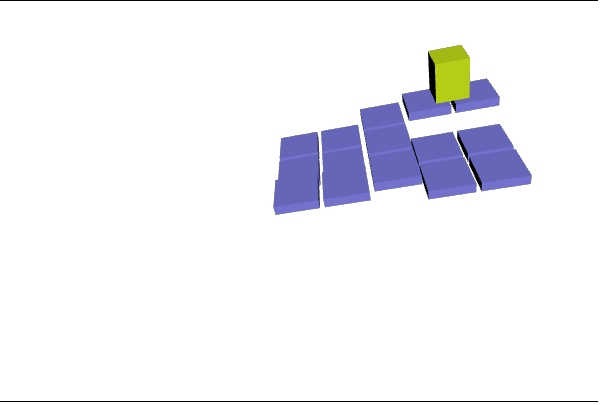
\includegraphics[scale=0.5]{ht1.png}
\end{figure}

\begin{figure}
\centering
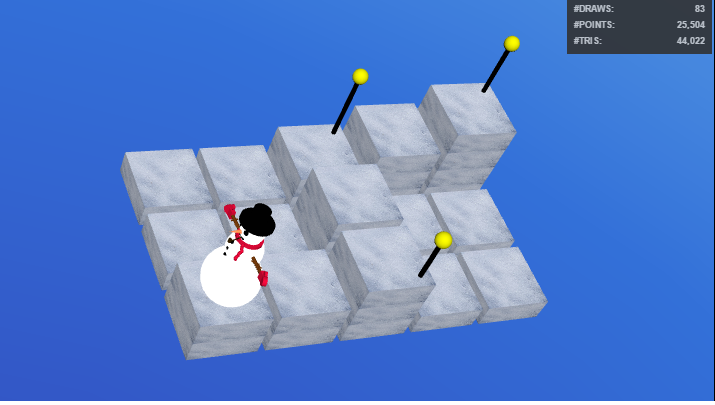
\includegraphics[scale=0.5]{ht2.png}
\end{figure}

\chapter{Conclusões}
Com a realizaçao deste projecto foi nos proporcionado uma oportunidade de adquirir novos conhecimentos e desenvolver outros pre-existentes na linguagem de Haskell e HTML, dando nos bases essenciais para o desenvolvimento de futuros projectos pessoais ou escolares nesta area. Para alem desta vertente mais tecnica este trabalho foi importante para compreender a importancia em trabalho de equipa e adequada do nosso tempo. 

\end{document}